\section{Visual System}
\label{sect:vision}

The robot visual system employs log-polar images as in \cite{sandini80retinalike}. The log-polar transformation, applied in this case to the traditional rectangular images coming from the cameras, mimics the distribution of the photoreceptors in the retina and the topological mapping from the retina to the primary visual cortex. Log-polar images have a small central area with maximum resolution (fovea) and a continuously decreasing number of pixels moving toward the periphery. 
Humans and primates move the eyes to take high resolution snapshots of important points in the environment. Likewise, depending on the task at hand, the robot has to move the cameras and place the fovea at interesting locations in the visual scene. In our system the selection of these locations is carried out by the visual attention system.
%In humans and primates there is the need to move the sensor to take high resolution snapshots of important points in the environment. Likewise, in order to acquire information from the environment, the robot has to move the cameras and place the fovea at interesting locations in the visual scene possibly according to the task at hand. In other words there is the need to have a module that selects information for further visual processing.

In addition, another important requirement for a visual system apt to guide manipulation is that of segmenting objects from a possibly cluttered background. That is, we need both the localization of the object and its segmentation. The problem of segmentation is directly related to the problem of defining what an object is, that is to define which properties distinguish an object from the background.

Our definition of ``objecthood'' is created in two steps:
\begin{itemize}
\item the selection of a set of visual features that can characterize any object of a certain set and allow segmenting it from the background;
\item the selection of a criterion for grouping features that segment and identify the objects uniquely;
\end{itemize}
\noindent In practice, we selected certain features and a method for deciding when a specific feature belongs to an object. The features we chose for our implementation are {\em colored blobs} while the criterion is a consequence of the action of the robot onto objects. In fact, by grasping an object the robot has the possibility of observing it at will from many points of view and with different backgrounds. It is consequently easy to imagine a procedure that selects the constant features across consecutive views of the same object.

By selecting blobs as features we do not propose to directly define what an object is, but rather to consider a sort of ``proto-objects''. They are a step above the mere features (e.g. edges), possessing some but not all the characteristics of an object; ``proto-objects'' in this view are clusters of points on the image ``naturally'' grouped together. The idea of proto-objects has its roots in psychological \cite{pylyshyn01indexes} and neurobiological literature. In fact it has been proposed that the synchronization of visual cortical neurons can be the carrier of the perceptual grouping phenomenon \cite{eckhorn88coherent,gray89oscillatory}.
In our implementation, we decided that the grouping acted on color and intensity information; this leads to the extraction of colored blobs as we mentioned earlier. 

To simulate the results of the process of grouping, we employed the watershed transform (rainfalling variant) \cite{smet00rainfalling} on the edge map resulting from a preliminary feature extraction stage. As a consequence the image is segmented in regions of either constant color or constant color gradient. A segmentation of this type has been demonstrated to happen in humans before the attention is deployed to the scene \cite{driver00segmentation}.

Following our definitions, the identity of an object cannot be known unless some other knowledge is inserted into the system. One possible route for acquiring this knowledge autonomously is by means of action. The robot can go beyond the concept of proto-objects and learn a model of the objects it manipulates. In particular, objects are seen here as a collection of proto-objects and their spatial relations. During manipulation the robot builds a statistical description of the blobs that are part of the object. Later on, the robot computes the probability that the set of blobs currently fixated are originated by the sameo object to identify and segment it. The complete description of the visual attention model and segmentation procedure can be found in \cite{orabona05object}.

The segmentation mask is used together with a binocular disparity estimation algorithm to extract three-dimensional information about the object.
This mask defines a region of interest on which the disparity algorithm computes a depth map. The spatial orientation of the object guides the behavior of the robot.
% The mask defines a region of interest around the object, where a depth map is estimated, and eventually the orientation in space of the object can be extracted and used to guide the behavior of the robot.

In order to achieve a good detection of the object orientation, we developed a fast and robust binocular disparity estimation algorithm that works at nearly frame rate. The algorithm is based on the work by Van Meerbergen et al. \cite{merrbergen02stereo}; in short it computes all possible matches between pixels in a scanline and builds a graph by assigning a cost to each position pair and each occlusion. The disparity map is computed by searching the optimal path on the graph by using dynamic programming.

With respect to the original formulation of the algorithm we relaxed the hypothesis of similar extension (over the scanline) of the pixel patterns: something that makes sense when the cameras are quasi-parallel, but that on the other hand fails dramatically when the cameras are converging and the objects are very close compared to the interocular distance.
The consequence is that a surface can be very different in shape between the two images of the stereo pair. As a result a short sequence of pixels in one image can match a long one in the other.

Each node of the graph represents a pixel pair, one on the left scanline $(L_x)$ and one on the right one $(R_y)$, starting from the nodes containing either $(L_0)$ or $(R_0)$ or both (the first pixels of the scanline) and ending with the nodes containing ${L_N}$, ${R_N}$ or both, where N is the length in pixels of the scanline. Each node is connected to all the following nodes according to these rules:

\begin{enumerate}
	\item \textit{Disparity Range:} $\delta_{min}\leq x-y \leq \delta_{max}$
	\item \textit{Ordering:} Given another pair $(L_{x'},R_{y'})$, if $x'\geq x$ then $y'\geq y$, assuming that there cannot be duplicate nodes
	\item \textit{Continuity:} the nodes following $(L_x,R_y)$ are all the nodes containing $(L_{x+1})$ or $(R_{y+1})$ that respect the previous two constraints
\end{enumerate}

\noindent Each arc has an associated cost:
	\[c=\left|lum(L_x)-lum(R_y)\right|+k\beta+\alpha
\]

\noindent where $lum$ represents the luminance of a pixel, $\beta$ is a cost (linear) associated to disparity jumps (if a node has disparity $\delta_i$ and the following one has disparity $\delta_j$, then $k=|\delta_i-\delta_j|$) and $\alpha$ takes into account the differences along the vertical dimension (to penalize large discontinuities in the final disparity map). Once the graph is built, the minimum cost to traverse it from beginning to end is found using dynamic programming. The disparity map is then constructed by considering the pairing of pixels along the minimum cost path. An example of the construction of the graph when considering two successive levels is shown in figure \ref{fig-graph}.

\begin{figure}
	\centering
		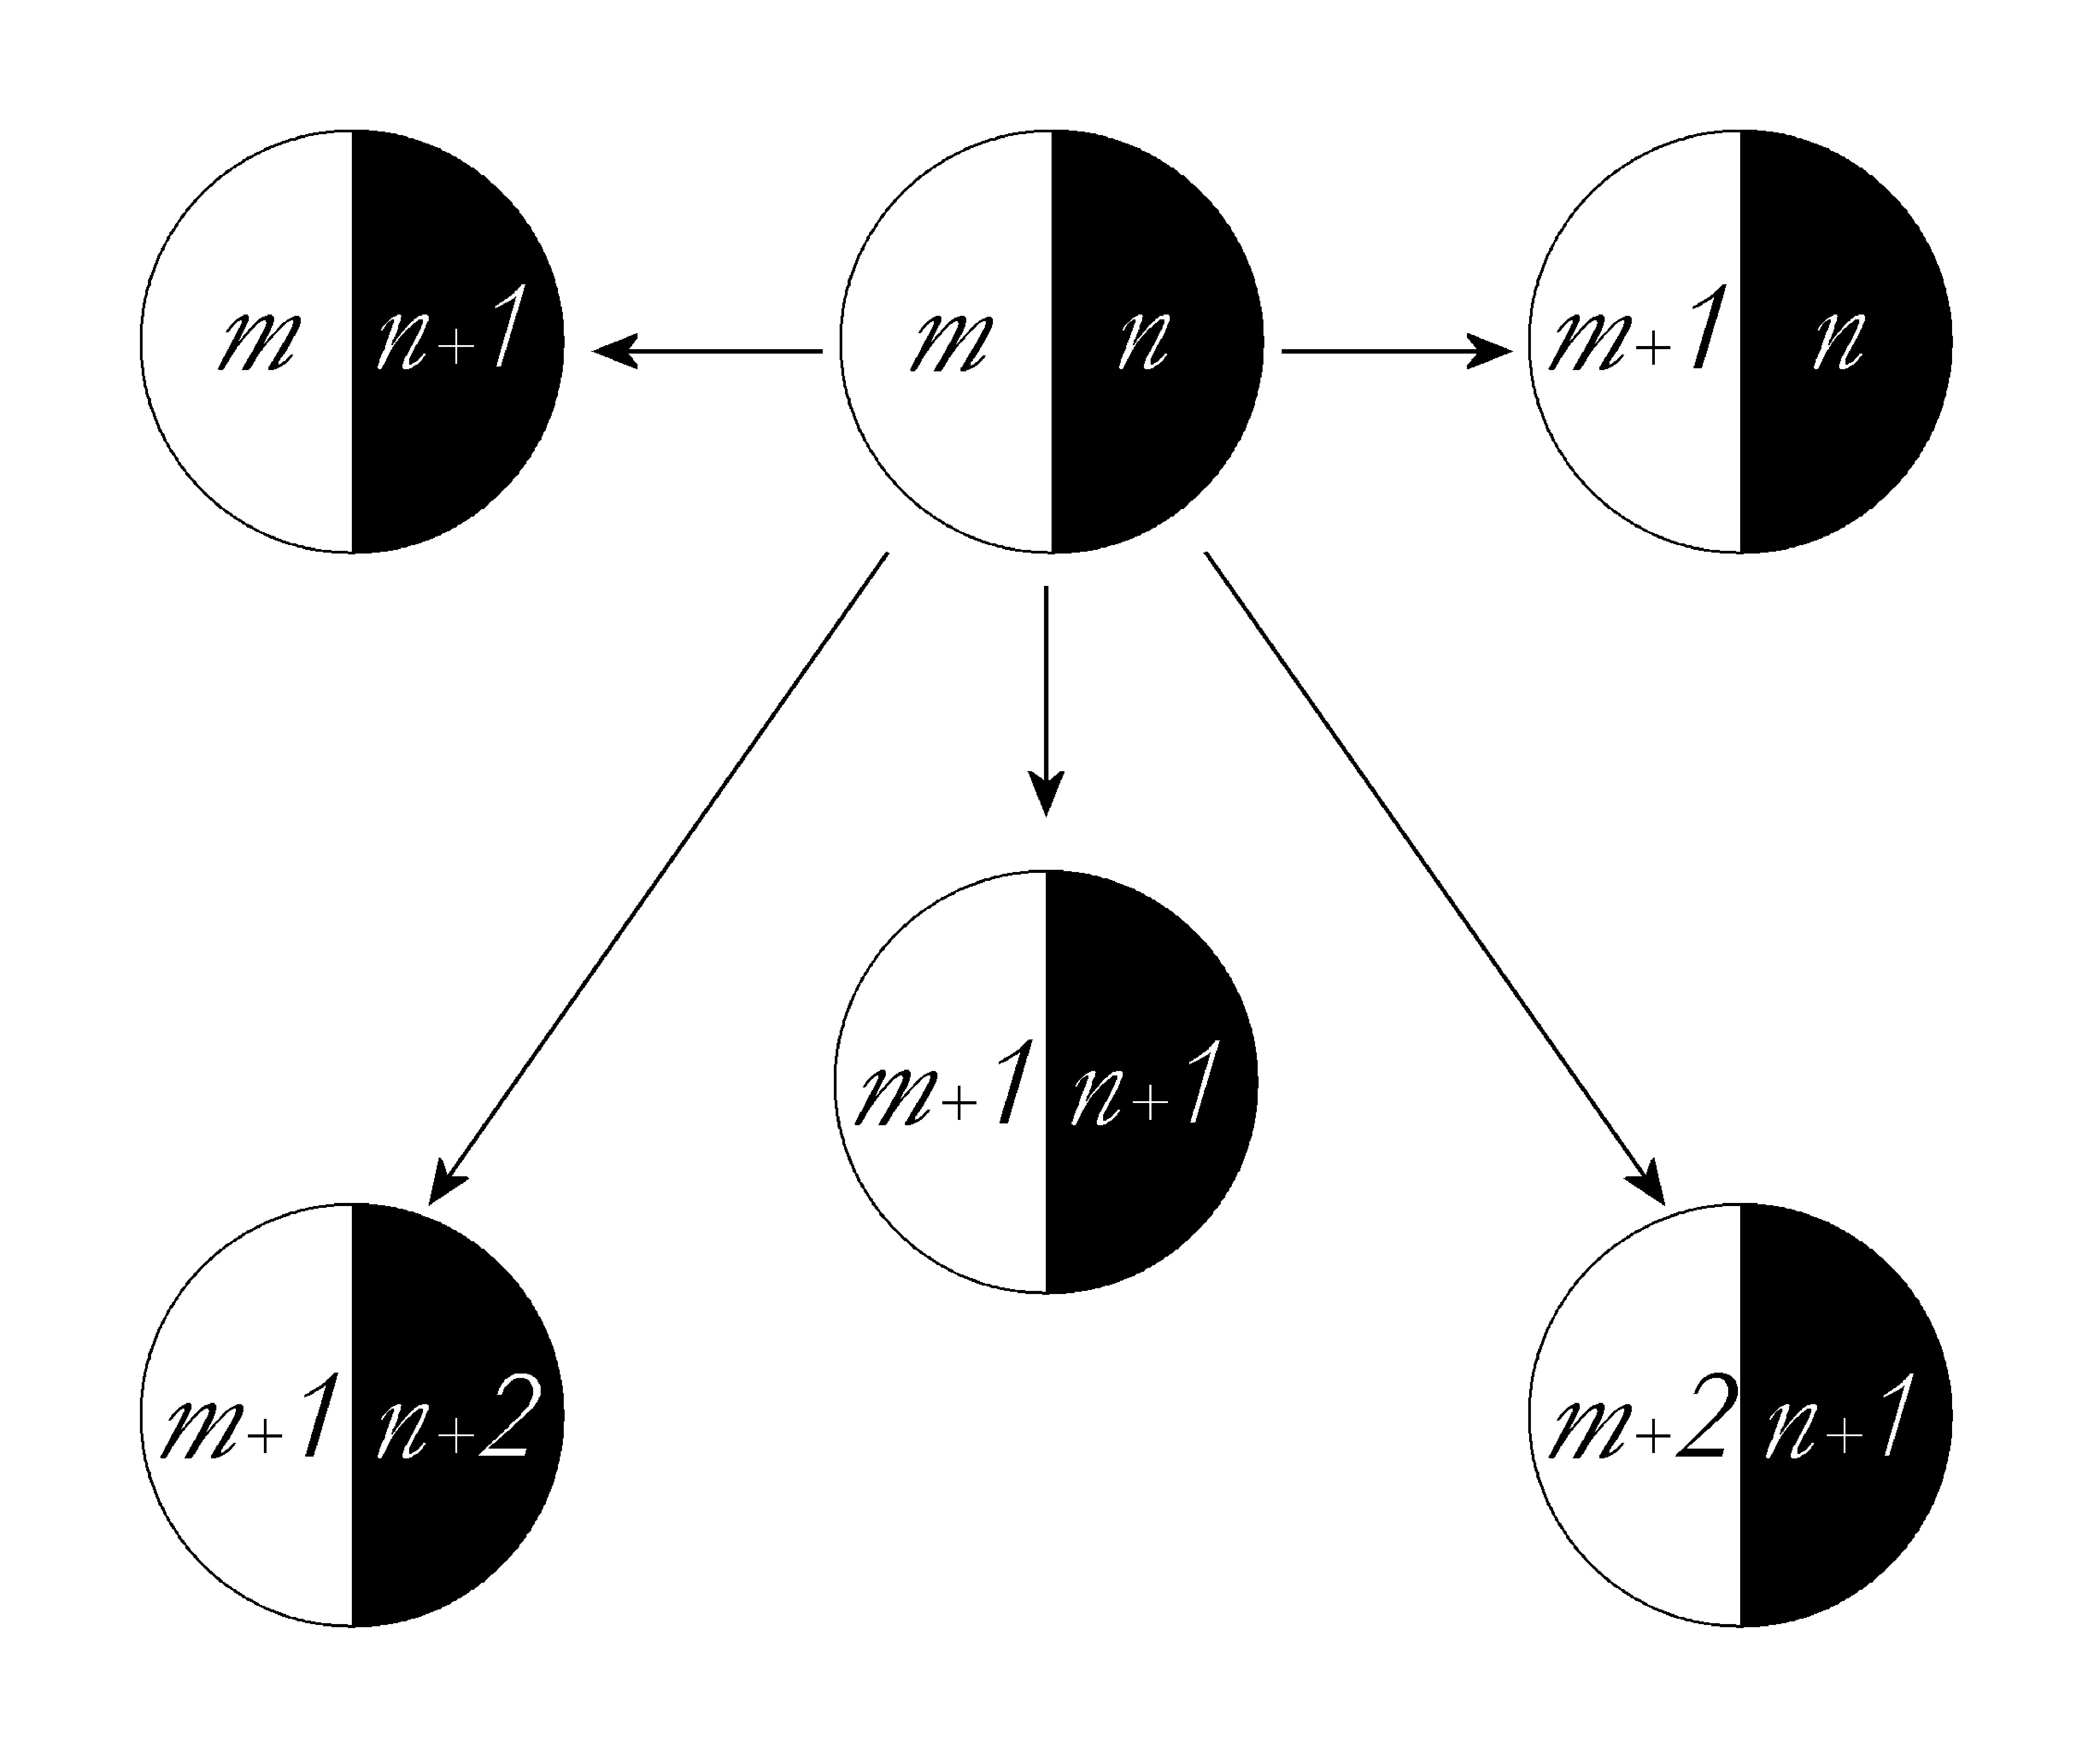
\includegraphics[width=2in]{graph.eps}
	\caption{A section of the graph: the columns have constant disparity $(m-n)$.}
	\label{fig-graph}
\end{figure}

The complexity of dynamic programming for each graph (i.e. each scanline) is $O(m)$, where $m$ is the total number of arcs in the graph and it is proportional to the length of the scanlines. To increase the performance of the algorithm we considered only the portion of the image around the object of interest. 
This reduces both {\em m} and the total number of lines to be processed. To increase the robustness, once computed the disparity map $D_{l-r}$ (displacement of the pixels in the left image compared to the ones in the right one), we used it to detect the object position on the right image, according to the formula: 
\begin{equation}D_{l-r}(x)=D_{r-l}(x-D_{l-r}(x))\end{equation}

This result is then used to segment the object on the right image. The images are swapped (left with right) and the disparity is computed again. This new estimate is finally used to validate and correct the previous one. An example of a masked depth map is shown in figure \ref{fig-disparity}.

\begin{figure}
\centering
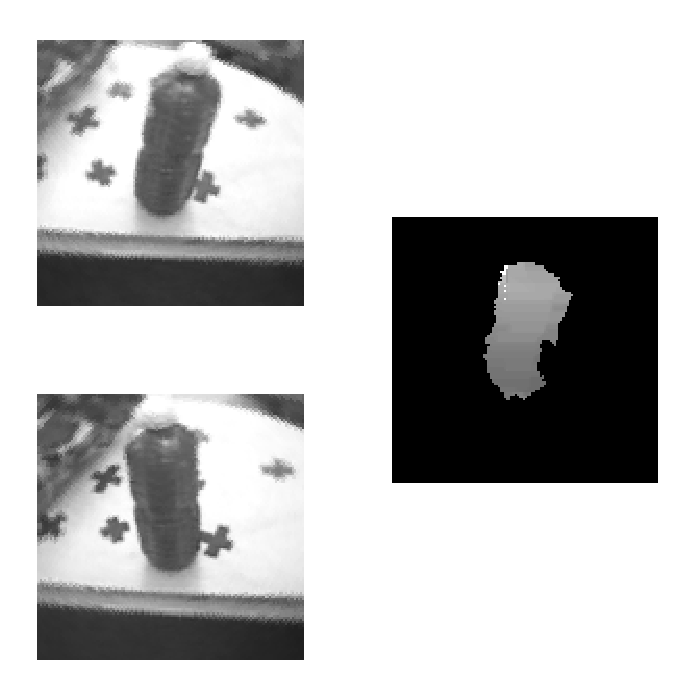
\includegraphics[width=2.5in]{disparity}
\caption{The Disparity Algorithm  Left: The Stereo Pair, Right: The Final Disparity Map, masked. The mask image comes from the attention algorithm.}
\label{fig-disparity}
\end{figure}

